\documentclass[twoside,11pt,a4paper]{article}

\usepackage{graphicx,curves,float,rotating}
\usepackage{amsmath, amssymb, latexsym}
\usepackage{amsopn}
\usepackage{theorem}
\usepackage{dcolumn}
\usepackage{hyperref}
\usepackage{enumerate}
\usepackage{sidecap}
\usepackage{subfigure}
\usepackage{pgfplots}
\usepackage[toc,page]{appendix}

\usepackage{tikz} % figures and diagrams
\usetikzlibrary{decorations.pathreplacing} % braces for tikz

\usepackage{xspace}
\makeatletter 
\DeclareRobustCommand\onedot{\futurelet\@let@token\@onedot}
\def\@onedot{\ifx\@let@token.\else.\null\fi\xspace}
\def\eg{{e.g}\onedot} \def\Eg{{E.g}\onedot}
\def\ie{{i.e}\onedot} \def\Ie{{I.e}\onedot}

% Define colors used for listings
\definecolor{dkgreen}{rgb}{0,0.6,0}
\definecolor{gray}{rgb}{0.5,0.5,0.5}
\definecolor{mauve}{rgb}{0.58,0,0.82}

\usepackage{listings}
\lstset{%
numbers=left,
frame=none,
basicstyle=\footnotesize\ttfamily,
numbers=left,
numberstyle=\tiny,
numbersep=15pt,tabsize=4,
flexiblecolumns=true,
keywordstyle=\color{blue},
commentstyle=\color{dkgreen}, 
stringstyle=\color{mauve},
numberstyle=\tiny\color{gray},
language=Matlab,
breaklines=true,
breakatwhitespace=true,
morekeywords={*,num,String,var,library,get,set} ,
}

\pagestyle{headings}
\textwidth 15cm
\textheight 23cm
\oddsidemargin 1cm
\evensidemargin 0cm
%\parindent 0mm

\begin{document}
\nocite{*} % Show references without needing to cite.

\pagestyle{empty}

\begin{center}

    RWTH Aachen University\\
    Chair of Computer Science 6\\
    Prof. Dr.-Ing. Hermann Ney\\[6ex]
    Selected Topics in Human Language Technology and Pattern Recognition WS 13/14\\[12ex]
   
    \LARGE
    \textbf{Introduction to Neural Networks} \\[6ex]
    \textit{David Stutz} \\[6ex]
    \Large
    February 10, 2014

    \vfill
    \Large Adviser: Pavel Golik
	    
\end{center}

\newpage
\newpage

\pagestyle{headings}
\tableofcontents
\listoftables
\listoffigures
\newpage
\pagestyle{empty}

\newpage
\pagestyle{headings}

\section{Abstract}

In this seminar paper we study artificial neural networks, their training and application to pattern recognition. We start by giving a general definition of artificial neural networks and introduce both the single-layer and the multilayer perceptron. After considering several activation functions we discuss network topology and the expressive power of multilayer perceptrons. The second section introduces supervised network training. Therefore, we discuss gradient descent and Newton's method for parameter optimization. We derive the error backpropagation algorithm for evaluating the gradient of the error function and extend this approach to evaluate its Hessian. In addition, the concept of regularization will be introduced. The third section introduces pattern classification. Using maximum likelihood estimation we derive the cross-entropy error function. As application, we train a two-layer perceptron to recognize handwritten digits based on the MNIST dataset.

\newpage

\section{Motivation}
\label{sec:motivation}

Theoretically, the human brain has a very low rate of operations per second when compared to a state of the art computer \cite[p.~28]{Haykin:2005}. Nevertheless, all computers are still outraveled by the human brain considering an important factor: \textbf{learning}. The human brain is able to learn how to perform certain tasks based on experience and prior knowledge.

\textbf{How to teach computers to learn?} To clarify the term ``learning'' in respect to computers we assume a set of training data $T = \{(x_n, t_n) : 1 \leq n \leq N\}$ for some $N \in \mathbb{N}$ and an arbitrary target function $g$ of which we know the target values $t_n := g(x_n)$. Our goal is to teach the computer a reasonably good approximation of $g(x)$ for $x$ in the domain of $g$. Many classification\footnote{The classification problem can be stated as follows: Given a $D$-dimensional input vector $x$ assign it to one of $C$ discrete classes (see section \ref{sec:pattern-recognition}).} and regression\footnote{The regression problem can be described as follows: Given a $D$-dimensional input vector $x$ predict the value of $C$ continuous target values.} problems can be formulated this way. The target function may even be unknown.

Considering noise within the given training data such that we only have a value $t_n \approx g(x_n)$ we require an additional property that we call \textbf{ability for generalization}. Solving the problem by interpolation may result in exact values $g(x_n)$ but may be a very poor approximation of $g(x)$ in general. This phenomenon is called over-fitting of the underlying training data.

\subsection{Historical Background and Bibliographical Notes}

In 1943 McCulloch and Pitts introduced the first mathematical models concerning networks of neurons we call artificial neural networks. But this first step did not include any results on network training \cite[p.~333-335]{DudaHartStork:2001}.

The first work on how to train similar networks was Rosenblatt's perceptron in 1958 which we discuss in section \ref{subsec:perceptron} \cite{Rosenblatt:1958}. Only ten years later Minsky and Papert showed that Rosenblatt's perceptron hat many limitations as we see in section \ref{subsec:expressive-power} and can only model linearly separable\footnote{Considering a classification problem as introduced in section \ref{sec:pattern-recognition} we say a set of data points is not linearly separable if the classes can not be separated by a hyperplane \cite[p.~179]{Bishop:2006}.} problems of classification \cite[p.~333-335]{DudaHartStork:2001}.

In \cite{RumelhartHintonWilliams:1986} Rumelhart, Hinton and Williams introduced the idea of error backpropagation for pattern recognition. In the late 80's it was shown that non linearly separable problems can be solved by multilayer perceptrons \cite{HornikStinchcombeWhite:1989}.

Weight decay was introduced in \cite{Hinton:1986}. A diagonal approximation of the Hessian was introduced in \cite{LeCun:1987}. A pruning method based on diagonal approximation of the Hessian is called Optimal Brain Damage and discussed in \cite{LeCunDenkerSolla:1990}. The exact evaluation of the Hessian is discussed in \cite{Bishop:1992}.

\newpage

\section{Neural Networks}
\label{sec:neural-networks}

An artificial neural network, also referred to as ``neural network'', is a set of interconnected processing units. A processing unit receives input from external sources and connected units and computes an output which may be propagated to other units. These units represent the neurons of the human brain which are interconnected by synapses \cite[p.~23-24]{Haykin:2005}.

A processing unit consists of a propagation rule and an activation function. The propagation rule determines the actual input of the unit by mapping the output of all direct predecessors and additional external inputs onto a single input value. The activation function is then applied on the actual input and determines the output of the unit. The output of the processing unit is also called activation. This is illustrated by figure \ref{fig:processing-unit} showing a single processing unit where $f$ denotes the activation function, $z$ the actual input and $y$ the output of the unit.

\begin{SCfigure}[2\sidecaptionrelwidth][t]
	\centering
	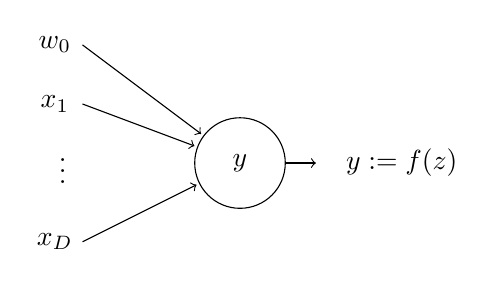
\begin{tikzpicture}[shorten >=1pt,->]
		\tikzstyle{unit}=[draw,shape=circle,minimum size=1.15cm]

		\node[unit](p) at (2,1){$y$};
		\node(dots) at (-0.25,1){\vdots};

		\draw (0,2.5) node[xshift=-10]{$w_0$} -- (p);
		\draw (0,1.75) node[xshift=-10]{$x_1$} --(p);
		\draw (0,0) node[xshift=-10]{$x_D$} -- (p);
		\draw (p) -- (3,1) node[xshift=30]{$y := f(z)$};
	\end{tikzpicture}
	\caption[Single processing units and its components.]{Single processing unit and its components. The activation function is denoted by $f$ and applied on the actual input $z$ of the unit to form its output $y = f(z)$. $x_1, \ldots, x_D$ represent input from other units within the network; $w_0$ is called bias and represents an external input to the unit. All inputs are mapped onto the actual input $z$ using the propagation rule.}
	\label{fig:processing-unit}
\end{SCfigure}

We distinguish input units and output units. Input units accept the input of the whole network and output units form the output of the network. Each input unit accepts a single input value $x$ and we set the output to $y := x$. Altogether, a neural network models a function $y(x)$ which dimensions are determined by the number of input and output units.
% For example figure \ref{fig:simple-network} shows a neural network with one input unit $p_1$ and one output unit $p_2$ such that it represents a function $y:\mathbb{R} \rightarrow \mathbb{R}$.

As to visualize neural networks we use directed graphs which we call network graphs. As illustrated in figure \ref{fig:processing-unit}, single processing units are represented by nodes and are interconnected by directed edges. The nodes of the graph are labeled according to the corresponding output.

%\begin{figure}[h]
%\begin{center}
%	\begin{tikzpicture}[shorten >=1pt]
%		\tikzstyle{unit}=[draw,shape=circle]
%
%		\node[unit](p1) at (0,0){$p_1$};
%		\node[unit](p2) at (1.5,0){$p_2$};
%
%		\draw[->] (p1) -- (p2);
%		\draw[->] (-1,0) node[xshift=-10]{$x$} -- (p1);
%		\draw[->] (p2) -- (2.5,0) node[xshift=6]{$y$};
%
%		\draw [decorate,decoration={brace,amplitude=10pt},xshift=-4pt,yshift=0pt] (-0.25,0.5) -- (2,0.5) node [black,midway,yshift=0.6cm]{neural network};
%	\end{tikzpicture}
%	\caption{Neural network with one input and one output unit.}
%	\label{fig:simple-network}
%\end{center}
%\end{figure}

\subsection{The Perceptron}
\label{subsec:perceptron}

As example we discuss Rosenblatt's perceptron which was introduced in 1958 \cite[p.~333-335]{DudaHartStork:2001}.
\begin{SCfigure}[12][b]
	\centering
    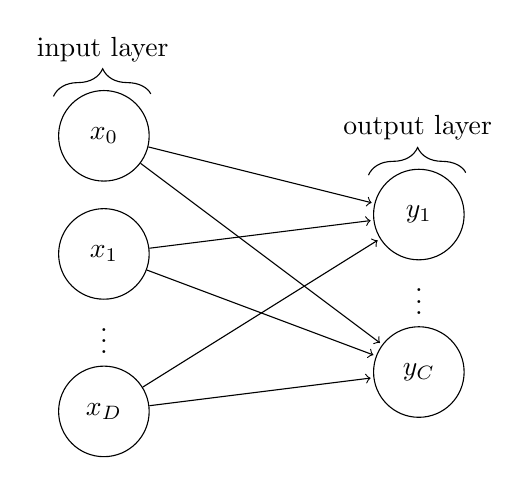
\begin{tikzpicture}[shorten >=1pt]
        \tikzstyle{unit}=[draw,shape=circle,minimum size=1.15cm]

        \node[unit](x0) at (0,3.5){$x_0$};
        \node[unit](x1) at (0,2){$x_1$};
        \node(dots) at (0,1){\vdots};
        \node[unit](xd) at (0,0){$x_D$};

        \node[unit](y1) at (4,2.5){$y_1$};
        \node(dots) at (4,1.5){\vdots};
        \node[unit](yc) at (4,0.5){$y_C$};

        \draw[->] (x0) -- (y1);
        \draw[->] (x0) -- (yc);

        \draw[->] (x1) -- (y1);
        \draw[->] (x1) -- (yc);

        \draw[->] (xd) -- (y1);
        \draw[->] (xd) -- (yc);

        \draw [decorate,decoration={brace,amplitude=10pt},xshift=-4pt,yshift=0pt] (-0.5,4) -- (0.75,4) node [black,midway,yshift=+0.6cm]{input layer};
        \draw [decorate,decoration={brace,amplitude=10pt},xshift=-4pt,yshift=0pt] (3.5,3) -- (4.75,3) node [black,midway,yshift=+0.6cm]{output layer};
    \end{tikzpicture}
    \caption[Network graph of a perceptron with $D$ input units and $C$ output units.]{The perceptron consists of $D$ input units and $C$ output units. All units are labeled according to their output: $y_i = f(z_i)$ in the case of output units; $x_i$ in the case of input units. The input values $x_i$ are propagated to each output unit using the weighted sum propagation rule. The additional input value $x_0 := 1$ is used to include the biases as weights. As suggested in section \ref{subsec:layered-networks} the units are assembled in layers.}
    \label{fig:perceptron}
\end{SCfigure}
The perceptron consists of $D$ input units and $C$ output units. Every input unit is connected to every output unit as shown in figure \ref{fig:perceptron}. For $1 \leq i \leq C$ the $i^{\text{th}}$ output unit computes the output
\begin{align}
y_i = f(z_i) \text{ with } z_i = \sum _{k=1} ^D w_{ik} x_k + w_{i0}
\end{align}
where $x_j$ is the input of the $j^{\text{th}}$ input unit. In this case the propagation rule is the weighted sum over all inputs with weights $w_{ik}$ and biases $w_{0k}$. The bias can be included as weight when considering an additional input $x_0 := 1$ such that the actual input $z_i$ can be written~as
\begin{align}
z_i = \sum _{k=0} ^d w_{ik} x_k\onedot
\end{align}

Throughout this paper we use the weighted sum as propagation rule for all units except the input units while activation functions may vary according to the discussion of the next section.

% The perceptron represents a function $y(x,w)$ where $w$ is the vector containing all variable weights. In the case of multiple input and output units we will use $y_i = y(x, w)$ to denote the output at the $i^{\text{th}}$ output unit.

\subsection{Activation Functions}

\begin{SCfigure}[\sidecaptionrelwidth][b!]
	\centering
    	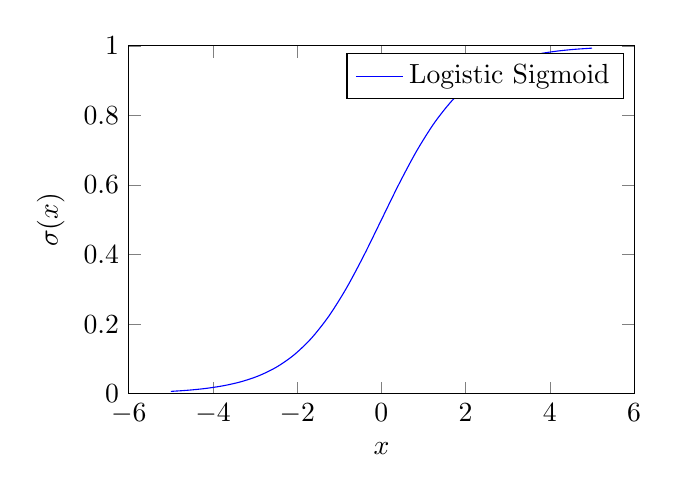
\begin{tikzpicture}
		\begin{axis}[width=8cm,height=6cm,ylabel=$\sigma(x)$,xlabel=$x$,ymin=0,ymax=1,xmin=-6,xmax=6]
			\addplot[blue,smooth] {1/(1+exp(-x))};
			\addlegendentry{Logistic Sigmoid}
		\end{axis}
	\end{tikzpicture}
    	\caption[The logistic sigmoid as activation function.]{The logistic sigmoid is a commonly used s-shaped activation function. It is both smooth and monotonic and allows an probabilistic interpretation as its range is limited to $[0,1]$.}
    	\label{fig:logistic-sigmoid}
\end{SCfigure}

The activation function determines the output of the unit. Often, a threshold function as for example the heaviside function
\begin{align}
h(z) = 
\begin{cases}
1  & \text{if } z \geq 0\\
0 & \text{if } z < 0
\end{cases}
\end{align}
is used \cite[p.~34-37]{Haykin:2005}. But in general we want the activation function to have certain properties. Network training using error backpropagation as discussed in section \ref{subsec:error-backpropagation} requires the activation function to be differentiable. In addition, we may want to use nonlinear activation functions as to increase the computational power of the network as discussed in section \ref{subsec:expressive-power} \cite[p.~307-308]{DudaHartStork:2001}.

A sigmoid function is a commonly used s-shaped function. The logistic sigmoid is given by
\begin{align}
\sigma(z) = \frac{1}{1 + \exp(-z)}
\end{align}
and shown in figure \ref{fig:logistic-sigmoid}. It can be considered as smooth version of the heaviside function. The softmax function is given by
\begin{align}
\sigma (z, i) = \frac{\exp(z_i)}{\sum _{k = 1} ^C \exp(z_k)}
\end{align}
where $C$ is the dimension of the vector $z$. Both functions are smooth and monotonic which means there are no additional local extrema. This is desirable for network training because multiple extrema within the activation function could cause additional extrema within the error surface \cite[p.~307-308]{DudaHartStork:2001}. In addition they allow a probabilistic interpretation which we use in section \ref{sec:pattern-recognition}. The derivatives of both the logistic sigmoid and the softmax function take preferable forms for implementation:
\begin{align}
\frac{\partial \sigma (z)}{\partial z} &= \sigma(z) (1 - \sigma(z))\text{,}\\
\frac{\partial \sigma (z, i)}{\partial z_j} &= \sigma(z, i) \left( \delta(i, j) - \sigma(z, j)\right)
\end{align}
where $\delta$ denotes the Kronecker delta\footnote{The Kronecker delta $\delta(i,j)$ equals $1$ if $j = i$ and is $0$ otherwise.}.

\subsection{Layered Networks}
\label{subsec:layered-networks}

Arranging the units in layers results in a layered network. Figure \ref{fig:perceptron} already introduced the perceptron as layered network. In this case we have a layer of input units and a layer of output units. We may add additional units organized in so called hidden layers. These units are called hidden units as they are not visible from the outside \cite[p.~43]{Haykin:2005}.

% Feed-forward topology can then be interpreted as follows: a unit in layer $i$ may only have an outgoing connection to a unit in layer $j$ if $j > i$. This includes connections skipping one or more layers.

For counting the number of layers we skip the input layer because there is no real processing taking place and no variable weights \cite[p.~229]{Bishop:2006}. Thus, the perceptron can be considered a single-layer perceptron without any hidden layers.

\subsection{Feed-Forward Networks}

% From the network diagram in figure \ref{fig:perceptron} we can consider a neural network as directed graph $(V,E,\omega)$ where $V$ is the set of processing units, $E$ the connections between them and $\omega: E \rightarrow \mathbb{R}$ a weight function.

Since we can model every neural network in the means of a network graph we get new neural networks by considering more complex network topologies \cite[p.229-231]{Bishop:2006}. We distinguish two network topologies:
\begin{description}
\item[Feed-forward] In a feed-forward topology we prohibit closed cycles within the network graph. This means that a unit in layer $p$ may only propagate its output to a unit in layer $l$ if $l > p$. Thus, the modeled function is deterministic.
\item[Recurrent] Recurrent networks allow closed cycles. A connection establishing a closed cycle within a network graph is called feedback connection.
%An obvious recurrent network is shown in figure \ref{fig:recurrent-network}.
\end{description}
%\begin{figure}[h]
%\begin{center}
%    \begin{tikzpicture}[shorten >=1pt]
%        \tikzstyle{unit}=[draw,shape=circle,minimum size=1.15cm]
%
%        \node[unit](x) at (0,3){$x$};
%
%        \node[unit](y) at (3,3){$y$};
%
%        \draw (x) edge[out=45,in=135,->] (y);
%        \draw (y) edge[out=215,in=325,->] (x);
%    \end{tikzpicture}
%    \caption{Simple recurrent network.}
%    \label{fig:recurrent-network}
%\end{center}
%\end{figure}
In this paper we consider feed-forward networks only. As demonstrated in figure \ref{fig:perceptron} the single-layer perceptron implements a feed-forward topology.

\subsection{Multilayer Perceptrons}
\label{subsec:multilayer-perceptron}

The multilayer perceptron has additional $L \geq 1$ hidden layers. The $l^{\text{th}}$ hidden layer consists of $m^{(l)}$ hidden units. The output value $y_{i}^{(l)}$ of the $i^{\text{th}}$ hidden unit within this layer is
\begin{align}
y_{i}^{(l)} = f\left(\sum _{k =1} ^{m^{(l-1)}} w_{ik}^{(l)} y_{k}^{(l-1)} + w_{i0}^{(l)}\right) \overset{y_{0}^{(l-1)} := 1}{=} f\left(\sum _{k = 0} ^{m^{(l-1)}} w_{ik}^{(l)} y_{k}^{(l-1)}\right)\onedot
\end{align}
Altogether, we count $(L+1)$ layers including the output layer where we set $D := m^{(0)}$ and $C := m^{(M+1)}$. Then $w_{ik}^{(l)}$ denotes the weighted connection between the $k^{\text{th}}$ unit of layer $(l-1)$ and the $i^{\text{th}}$ unit of layer $l$. Figure \ref{fig:twolayer-perceptron} shows a two-layer perceptron with $m := m^{(1)}$ units in its hidden layer. As previously mentioned, we added additional units $x_0 := y_0^{(1)} := 1$ to represent the biases.
\begin{SCfigure}[\sidecaptionrelwidth][t]
	\centering
	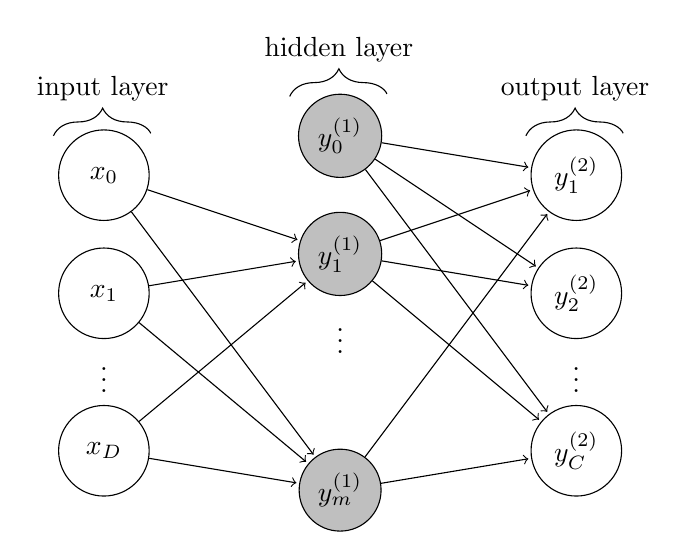
\begin{tikzpicture}[shorten >=1pt]
		\tikzstyle{unit}=[draw,shape=circle,minimum size=1.15cm]
		\tikzstyle{hidden}=[draw,shape=circle,fill=black!25]

		\node[unit](x0) at (0,3.5){$x_0$};
		\node[unit](x1) at (0,2){$x_1$};
		\node(dots) at (0,1){\vdots};
		\node[unit](xd) at (0,0){$x_D$};

		\node[hidden](h0) at (3,4){$y_0^{(1)}$};
		\node[hidden](h1) at (3,2.5){$y_1^{(1)}$};
		\node(dots) at (3,1.5){\vdots};
		\node[hidden](hm) at (3,-0.5){$y_m^{(1)}$};

		\node[unit](y1) at (6,3.5){$y_1^{(2)}$};
		\node[unit](y2) at (6,2){$y_2^{(2)}$};
		\node(dots) at (6,1){\vdots};	
		\node[unit](yc) at (6,0){$y_C^{(2)}$};

		\draw[->] (x0) -- (h1);
		\draw[->] (x0) -- (hm);

		\draw[->] (x1) -- (h1);
		\draw[->] (x1) -- (hm);

		\draw[->] (xd) -- (h1);
		\draw[->] (xd) -- (hm);

		\draw[->] (h0) -- (y1);
		\draw[->] (h0) -- (yc);
		\draw[->] (h0) -- (y2);

		\draw[->] (h1) -- (y1);
		\draw[->] (h1) -- (yc);
		\draw[->] (h1) -- (y2);

		\draw[->] (hm) -- (y1);
		\draw[->] (hm) -- (yc);

		\draw [decorate,decoration={brace,amplitude=10pt},xshift=-4pt,yshift=0pt] (-0.5,4) -- (0.75,4) node [black,midway,yshift=+0.6cm]{input layer};
		\draw [decorate,decoration={brace,amplitude=10pt},xshift=-4pt,yshift=0pt] (2.5,4.5) -- (3.75,4.5) node [black,midway,yshift=+0.6cm]{hidden layer};
		\draw [decorate,decoration={brace,amplitude=10pt},xshift=-4pt,yshift=0pt] (5.5,4) -- (6.75,4) node [black,midway,yshift=+0.6cm]{output layer};
	\end{tikzpicture}
	\caption[Network graph for a two-layer perceptron with $C$ input units, $D$ output units and $m$ hidden units.]{A two-layer perceptron with $C$ input units, $D$ output units and $m := m^{(1)}$ hidden units. Again, we introduced units $x_0 := 1$ and $y_0^{(1)} := 1$ to include the biases as weights. To distinguish units and weights with same indices in different layers, the number of the layer is written as superscript.}
	\label{fig:twolayer-perceptron}
\end{SCfigure}

In this paper we discuss the feed-forward multilayer perceptron as model for neural networks. The modeled function takes the form
\begin{align}
y(\cdot,w): \mathbb{R}^D \rightarrow \mathbb{R}^C, x \mapsto y(x,w) =
\begin{pmatrix}
y_1(x,w)\\
\vdots\\
y_C(x,w)
\end{pmatrix}
\end{align}
where $w$ is the vector comprising of all weights and $y_i(x,w) := y_i^{(L+ 1)}(x,w)$ is the output of the $i^{\text{th}}$ output unit.

\subsection{Expressive Power}
\label{subsec:expressive-power}

One of Minsky and Papert's results in 1969 showed that the single-layer perceptron has severe limitations one of which is called the Exclusive-OR (XOR) problem \cite[p.333-335]{DudaHartStork:2001}. As introduction we consider the target function $g$, which we want to model, given by
\begin{align}
g: \{0,1\}^2 \rightarrow \{0,1\}, x := (x_1, x_2) \mapsto 
\begin{cases}
1  & \text{if } x_1 = x_2 = 1\\
0 & \text{otherwise}
\end{cases}\onedot
\end{align}
Apparently, $g$ describes boolean AND. With $D = 2$ input units and $C = 1$ output unit using the $sgn(x)$ activation function, $g$ can be modeled by a single-layer perceptron:
\begin{align}
\label{eq:boolean-perceptron}
y = sgn(z) = sgn( w_{1} x_1 + w_{2} x_2 + w_{0})\onedot
\end{align}
Figure \ref{fig:boolean-perceptron} illustrates the corresponding network graph. By setting $z = 0$ we can interpret equation \eqref{eq:boolean-perceptron} as straight line in two-dimensional space:
\begin{align}
x_2 = - \frac{w_{1}}{w_{2}} x_1 - \frac{w_{0}}{w_{2}}\onedot
\end{align}
\begin{figure}[t]
\centering
\subfigure[Boolean AND (left) and boolean XOR (right) represented as classification problems.]{
    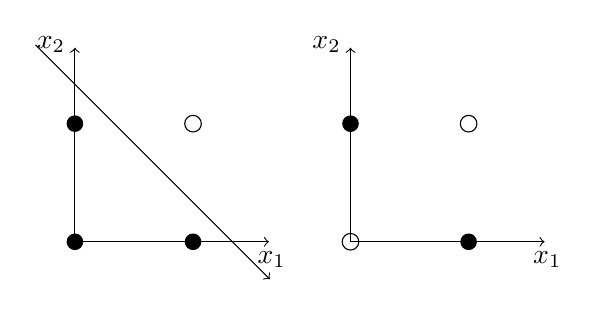
\begin{tikzpicture}[shorten >=1pt,->]
		\draw (0,0) -- (2.5,0) node[anchor=north]{$x_1$};
		\draw (0,0) -- (0,2.5) node[anchor=east]{$x_2$};
		\fill[black] (0,0) circle (3pt);
		\fill[black] (0,1.5) circle (3pt);
		\fill[black] (1.5,0) circle (3pt);
		\draw (1.5,1.5) circle (3pt);
		\draw[->] (-0.5,2.5) -- (2.5,-0.5);

		\draw (3.5,0) -- (6,0) node[anchor=north]{$x_1$};
		\draw (3.5,0) -- (3.5,2.5) node[anchor=east]{$x_2$};
		\draw (3.5,0) circle (3pt);
		\fill[black] (3.5,1.5) circle (3pt);
		\fill[black] (5,0) circle (3pt);
		\draw (5,1.5) circle (3pt);
	\end{tikzpicture}
	\label{fig:XOR}
}
\quad
\subfigure[Network graph of a single-layer perceptron modeling boolean AND.]{
    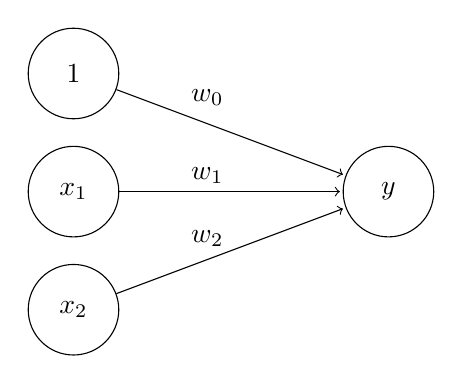
\begin{tikzpicture}[shorten >=1pt]
      		\tikzstyle{unit}=[draw,shape=circle,minimum size=1.15cm]

       	\node[unit](x0) at (0,3){$1$};
        	\node[unit](x1) at (0,1.5){$x_1$};
		\node[unit](x2) at (0,0){$x_2$};

        	\node[unit](y) at (4,1.5){$y$};

        	\draw[->] (x0) -- (y);
        	\draw[->] (x1) -- (y);
		\draw[->] (x2) -- (y);

		\node at (1.7,0.9){$w_2$};
		\node at (1.7,1.7){$w_1$};
		\node at (1.7,2.7){$w_0$};
    	\end{tikzpicture}
    	\label{fig:boolean-perceptron}
}
\caption[Single-layer perceptron for modeling boolean AND.]{Figure \ref{fig:XOR} shows both boolean AND and boolean XOR represented as classification problems. As we can see, boolean XOR is not linearly separable. A simple single-layer-perceptron capable of separating boolean AND is shown in figure \ref{fig:boolean-perceptron}.}
\label{fig:subfigureExample}
\end{figure}
A possible solution for modeling boolean AND is shown in figure \ref{fig:XOR}. But, as we can see, boolean XOR cannot be modeled by this single-layer perceptron. We say boolean XOR is not linearly separable\footnote{When considered as classification problem (see section \ref{sec:pattern-recognition}) we say the problem is not linearly separable if the classes can not be separated by a hyperplane \cite[p.~179]{Bishop:2006}.} \cite[p.~197-200]{Haykin:2005}.

This limitation can be overcome by adding at least one additional hidden layer. Theoretically, a two-layer perceptron is capable of modeling any continuous function when using appropriate nonlinear activation functions. This is a direct consequence of Kolmogorov's theorem. It states that for every continuous function $f : [0,1]^D \rightarrow \mathbb{R}$ there exist continuous functions $\psi _j : [0,1] \rightarrow \mathbb{R}$ such that $f$ can be written in the form
\begin{align}
f(x_1, \ldots, x_D) = \sum _{j = 0} ^{2D} g_f\left(\sum _{k = 1} ^D w_k \psi _j (x_k)\right)\onedot
\end{align}
But as of \cite[p.~137-140]{Bishop:1995} the function $g_f$ is dependent on $f$ and the theorem is not applicable if the functions $\psi _j$ are required to be smooth. In most applications we do not know the target function. And  the theorem says nothing about how to find the functions $\psi _j$. It simply states the existence of such functions. Thus, the theorem is not of much practical use for network design \cite[p.~287-288]{DudaHartStork:2001}. Nevertheless, the theorem is important as it states that theoretically we are able to find an optimal solution using one hidden layer. Otherwise, we could end up with a problem for which we cannot find a solution using a multilayer perceptron \cite[p.~234-235]{Haykin:2005}.

\newpage

\section{Network Training}
\label{sec:network-training}

Network training describes the problem of determining the parameters to model the target function. Therefore, we use a set of training data representing the initial knowledge of the target function. Often the target function is unknown and we only know the value of the function for specific data points.

Depending on the training set we consider three different learning paradigms \cite[p.~85-88]{Haykin:2005}:
\begin{description}
\item[Unsupervised learning] The training set provides only input values. The neural network has to find similarities by itself.
\item[Reinforcement learning] After processing an input value of the training set the neural network gets feedback whether the result is considered good or bad.
\item[Supervised learning] The training set provides both input values and desired target values (labeled training set).
\end{description}

Although the human brain mostly learns by reinforcement learning (or even unsupervised learning), we discuss supervised learning only. Let $T := \{(x_n, t_n) : 1 \leq n \leq N\}$ be a training set where $x_n$ are input values and $t_n$ the corresponding target values. As for any approximation problem we can evaluate the performance of the neural network using some distance measure between approximation and target function.

\subsection{Error Measures}
\label{subsec:error-measures}

We discuss mainly two error measures. The sum-of-squared error function takes the form
\begin{align}
E (w) = \sum _{n = 1} ^N E_n (w) = \frac{1}{2} \sum _{n = 1} ^N \sum _{k = 1} ^C (y_k(x_n,w) - t_{nk})^2
\end{align}
where $t_{nk}$ denotes the $k^{\text{th}}$ entry of the $n^{\text{th}}$ target value. The cross-entropy error function is given by
\begin{align}
E(w) = \sum _{n = 1} ^N E_n (w) = - \sum _{n = 1} ^N \sum _{k = 1} ^C t_{nk} \log(y_k(x_n, w))\onedot
\end{align}

For further discussion we note that by using $y_i(x_n,w) = f (z_i)$ the derivatives of both error functions with respect to the actual input $z_i^{(L+1)}$ of the $i^{\text{th}}$ output unit take the form
\begin{align}
\frac{\partial E_n}{\partial z_i^{(L+1)}} = \frac{\partial E_n}{\partial y_i^{(L+1)}} \frac{\partial y_i^{(L+1)}}{\partial z_i^{(L+1)}} = y_i(x_n,w) - t_{ni}\onedot
\end{align}
Here we use the softmax activation function for the cross-entropy error function and the identity as activation function for the sum-of-squared error function \cite[p.~230-231,236-240]{Bishop:1995}.

\subsection{Training Approaches}

Given an error function $E(w) = \sum _{n = 1} ^N E_n (w)$ we distinguish mainly two different training approaches \cite[p.~293-295]{DudaHartStork:2001}:
\begin{description}
\item[Stochastic training] Randomly choose an input value $x_n$ and propagate it through the network. Update the weights based on the error $E_n(w)$.
\item[Batch training] Go through all input values $x_n$ and compute $y(x_n,w)$. Update the weights based on the overall error $E(w) = \sum _{n = 1} ^N E_n(w)$.
\end{description}
Instead of choosing an input value $x_n$ at random we could also select the input values in sequence leading to sequential training. As of \cite[p.~240-241]{Bishop:2006} stochastic training is considered to be faster especially on redundant training sets.

\subsection{Parameter Optimization}
\label{subsec:parameter-optimization}

The weight update in both approaches is determined by a parameter optimization algorithm which tries to minimize the error. The error $E(w)$ can be considered as error surface above the weight space. In general, the error surface is a nonlinear function of the weights and may have many local minima and maxima. We want to find the global minimum. The necessary criterion to find a minimum is
\begin{align}
\nabla E (w) = 0
\end{align}
where $\nabla E$ denotes the gradient of the error function $E$ evaluated at point $w$.

As an analytical solution is usually not possible we use an iterative approach for minimizing the error. In each iteration step we choose an weight update $\Delta w[t]$ and set
\begin{align}
w[t + 1] = w[t] + \Delta w[t]
\end{align}
where $w[t]$ denotes the weight vector $w$ in the $t^{\text{th}}$ iteration and $w[0]$ is an appropriate starting vector. Optimization algorithms differ in choosing the weight update $\Delta w[t]$ \cite[p.~254-256]{Bishop:1995}. Before discussing two common optimization algorithms, we discuss the case of linear units and the problem of choosing a good starting vector $w[0]$.

\subsubsection{Linear Units}

In the case of a single-layer perceptron with linear output units and sum-of-squared error we obtain a linear problem. Thus, we can determine the weights exactly using singular value decomposition \cite[p.~259-260]{Bishop:1995}.

When considering a multilayer perceptron with linear output units and nonlinear hidden units we can at least split up the problem of minimization. The weights in the output layer can be determined exactly using singular value decomposition whereas the weights in the hidden layers can be optimized using an iterative approach. Note that every time the weights of the nonlinear layers are updated the exact solution for the weights in the output layer has to be recomputed \cite[p.~259-260]{Bishop:1995}.

\subsubsection{Weight Initialization}

Following \cite[p.~311-312]{DudaHartStork:2001} we want to get a starting vector $w$ such that we have fast and uniform learning, that is all components learn more or less equally fast. Assuming sigmoidal activation functions the actual input of a unit should neither be too large causing $\sigma'(z)$ to be very small nor be too small such that $\sigma(z)$ is approximately linear. Both cases will result in slow learning. For the logistic sigmoid an acceptable value for the unit input is of unity order \cite[p.~260-262]{Bishop:1995}. Thus, we choose all weights randomly from the same distribution such that
\begin{align}
- \frac{1}{\sqrt{m^{(l - 1)}}} < w_{ij}^{(l)} < \frac{1}{\sqrt{m^{(l - 1)}}}
\end{align}
for the weights in layer $l$. Assuming a normal distribution with zero mean and unity variance for the inputs of each unit we get on average the desired actual input of unity order \cite[p.~311-312]{DudaHartStork:2001}.

\subsubsection{Gradient Descent}

Gradient descent is a basic first-order optimization algorithm. This means that in every iteration step we use information about the gradient $\nabla E$ at the current point. In iteration step $[t + 1]$ the weight update $\Delta w[t]$ is determined by taking a step into the direction of the negative gradient at position $w[t]$ such that
\begin{align}
\Delta w[t] = - \gamma \frac{\partial E}{\partial w[t]}
\end{align}
where $\gamma$ is called learning rate. Gradient descent can be used both for batch training and stochastic training\cite[p.~240-241]{Bishop:2006}. In the case of stochastic training we choose
\begin{align}
\Delta w[t] = - \gamma \frac{\partial E_n}{\partial w[t]}
\end{align}
as weight update.

\subsubsection{Momentum}

\begin{figure}[t!]
	\centering
	\subfigure[High learning rate.]{
    		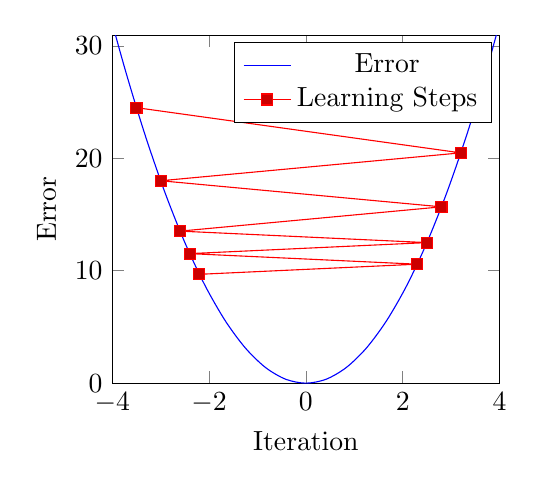
\begin{tikzpicture}
			\begin{axis}[height=6cm,width=6.5cm,ylabel=Error,xlabel=Iteration,xmin=-4,xmax=4,ymin=0]
				\addplot[blue,smooth] {2*x^2};
				\addlegendentry{Error}
				\addplot+[red] coordinates{(-3.5,24.5)(3.2,20.48)(-3,18)(2.8,15.68)(-2.6,13.52)(2.5,12.5)(-2.4,11.52)(2.3,10.58)(-2.2,9.68)};
				\addlegendentry{Learning Steps}
			\end{axis}
		\end{tikzpicture}
		\label{subfig:momentum-high}
	}
	\subfigure[Low learning rate.]{
		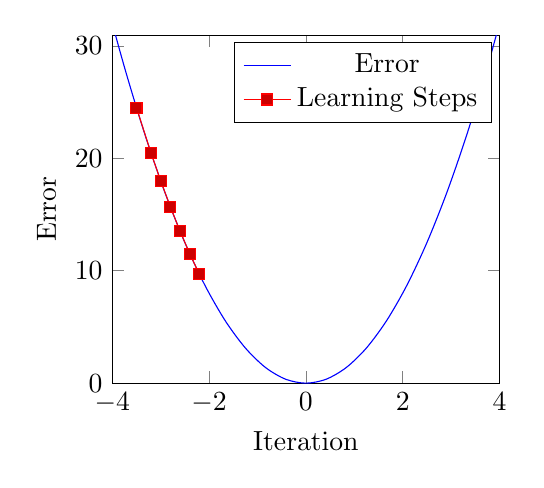
\begin{tikzpicture}
			\begin{axis}[height=6cm,width=6.5cm,ylabel=Error,xlabel=Iteration,xmin=-4,xmax=4,ymin=0]
				\addplot[blue,smooth] {2*x^2};
				\addlegendentry{Error}
				\addplot+[red] coordinates{(-3.5,24.5)(-3.2,20.48)(-3,18)(-2.8,15.68)(-2.6,13.52)(-2.4,11.52)(-2.2,9.68)};
				\addlegendentry{Learning Steps}
			\end{axis}
		\end{tikzpicture}
		\label{subfig:momentum-low}
	}
    	\caption[The learning rate and its influence on the rate of convergence.]{When using a large learning rate the weight updates in each iteration tend to overstep the minimum. This causes oscillation around the minimum. This observation is illustrated by figure \ref{subfig:momentum-high}. Choosing the learning rate too low will result in a slow convergence to the minimum as shown in figure \ref{subfig:momentum-low}. Both scenarios are visualized using a quadratic function we seek to minimize.}
    	\label{fig:momentum}
\end{figure}
The choice of the learning rate can be crucial. We want to choose the learning rate such that we have fast learning but avoid oscillation when choosing the learning rate too large \cite[p.~267-268]{Bishop:1995}. Both cases are illustrated by figure \ref{fig:momentum} where we seek to minimize a convex quadratic function. One way to reduce oscillation while using a high learning rate as described in \cite[p.~267-268]{Bishop:1995} is to add a momentum term. Then the change in weight is dependent on the previous change in weight such that
\begin{align}
\Delta w[t] = - \gamma \frac{\partial E}{\partial w[t]} + \lambda \Delta w[t - 1]
\end{align}
where $\lambda$ is called momentum parameter. %Evidently $\lambda$ should lie in the range $0 \leq \lambda \leq 1$.

\subsubsection{Enhanced Gradient Descent}

There is still a serious problem with gradient descent: how to choose the learning rate (and the momentum parameter). Currently, we are required to choose the parameters manually. Because the optimal values are dependent on the given problem, an automatic choice is not possible.

We discuss a simple approach on choosing the learning rate automatically considering no momentum term. Let $\gamma [t]$ denote the learning rate in the $t^{\text{th}}$ iteration. Then we have a simple criterion on whether the learning rate was chosen too large: If the error has increased after the weight update we may have overstepped the minimum. Then we can undo the weight update and choose a smaller learning rate until the error decreases \cite[p.~268-272]{Bishop:1995}. Thus, we have
\begin{align}
\gamma [t + 1] = 
\begin{cases}
\rho \cdot \gamma [t] & \text{if } E(w[t + 1]) < E(w[t]) \\
\mu \cdot \gamma [t] & \text{if } E(w[t + 1]) > E(w[t])
\end{cases}
\end{align}
where the update parameters can be chosen as suggested in \cite[p.~268-272]{Bishop:1995}: set $\rho := 1.1$ to avoid frequent overstepping of the minimum; set $\mu := 0.5$ to ensure fast recovery to taking a step which minimizes the error.

% \subsubsection{Second Order Methods}
%
% Although gradient descent has been improved in many ways it is considered a poor optimization algorithm as pointed out in \cite[p.~268-269]{Bishop:1995} and \cite[p.~240-241]{Bishop:2006}. But optimization is a widely studied area and, thus, there are more efficient algorithms. Conjugate gradients makes implicit use of second order information. Newton's Method or so called Quasi-Newton Methods explicitly use the Hessian of the error function in each iteration step. Some of these algorithms are described in detail in \cite[p.~274-290]{Bishop:1995}.

\subsubsection{Newton's Method}

Although gradient descent has been improved in many ways it is considered a poor optimization algorithm as pointed out in \cite[p.~268-269]{Bishop:1995} and \cite[p.~240-241]{Bishop:2006}. But optimization is a widely studied area and, thus, there are more efficient algorithms. Conjugate gradients makes implicit use of second order information. Newton's method or so called quasi-Newton methods explicitly use the Hessian of the error function in each iteration step. Some of these algorithms are described in detail in \cite[p.~274-290]{GillMurrayWright:1997}. We discuss the general idea of Newton's method.

Newton's method is an iterative optimization algorithm based on a quadratic approximation of $E$ using the Taylor series. Let $H(w[t])$ denote the Hessian of the error function evaluated at $w[t]$. Then, by taking the first three terms of the Taylor series\footnote{In general, the Taylor series of a smooth function $f$ at point $x_0$ is given by \begin{align}T(x) = \sum _{k = 0} ^\infty \frac{f^{(k)} (x_0)}{k!} (x - x_0)^k\onedot\end{align}}, we obtain a quadratic approximation of $E$ around the point~$w[t]$ \cite[p.~105-106]{GillMurrayWright:1997}:
\begin{align}
\tilde{E}(w[t] + \Delta w[t]) & = E(w[t]) + \nabla E(w[t])^{tr} \Delta w[t] + \frac{1}{2} (\Delta w[t])^{tr} H(w[t]) \Delta w[t]\onedot
\end{align}
We want to choose the weight update $\Delta w[t]$ such that the quadratic approximation $\tilde{E}$ is minimized. Therefore, the necessary criterion gives us:
\begin{align}
\nabla \tilde{E}(w[t] + \Delta w[t]) & = \nabla E(w[t]) + H(w[t]) \Delta w[t] \overset{!}{=} 0\onedot
\end{align}
The solution is given by
\begin{align}
\label{eq:newton-update}
\Delta w[t] = - \gamma H(w[t])^{-1} \nabla E(w[t])
\end{align}
where $H(w[t])^{-1}$ is the inverse of the Hessian at point $w[t]$. Because we use a quadratic approximation, equation \eqref{eq:newton-update} needs to be applied iteratively. When choosing $w[0]$ sufficiently close to the global minimum of $E$, Newton's method converges quadratically \cite[p.~105-106]{GillMurrayWright:1997}.

Nevertheless, Newton's method has several drawbacks. As we see later, the evaluation of the Hessian matrix and its inversion is rather expensive\footnote{The inversion of a $n \times n$ matrix usually requires $\mathcal{O}(n^3)$ operations.}. In addition, the Newton step in equation \eqref{eq:newton-update} may be a step in the direction of a local maximum or saddle point. This may happen if the Hessian matrix is not positive definite \cite[p.~285-287]{Bishop:1995}.

\subsection{Error Backpropagation}
\label{subsec:error-backpropagation}

Error backpropagation describes an efficient algorithm to evaluate $\nabla E_n$ for multilayer perceptrons using differentiable activation functions.

Following \cite[p.~241-245]{Bishop:2006} we consider the $i^\text{th}$ output unit first. The derivative of an arbitrary error function $E_n$ with respect to the weight $w_{ij}^{(L+1)}$ is given by
\begin{align}
\label{eq:partial-factors}
\frac{\partial E_n}{\partial w_{ij}^{(L+1)}} \underset{rule}{\overset{\text{chain-}}{=}} \frac{\partial E_n}{\partial z_i^{(L+1)}} \frac{\partial z_i^{(L+1)}}{\partial w_{ij}^{(L+1)}}
\end{align}
where $z_i^{(L+1)}$ denotes the actual input of the $i^\text{th}$ unit within the output layer. Using the chain rule, the first factor in equation \eqref{eq:partial-factors} can be written as
\begin{align}
\label{eq:output-first-factor}
\delta _i ^{(L+1)} := \frac{\partial E_n}{\partial z_i^{(L+1)}} & \underset{rule}{\overset{\text{chain-}}{=}} \frac{\partial E_n}{\partial y_i^{(L+1)}} \frac{\partial y_i^{(L+1)}}{\partial z_i^{(L+1)}}\notag\\
& = \frac{\partial E_n}{\partial y_i^{(L+1)}} f'\left(z_i^{(L+1)}\right)
\end{align}
where $\delta _i ^{(L+1)}$ is often called error and describes the influence of the $i^\text{th}$ output unit on the total error $E_n$. The second factor of equation \eqref{eq:partial-factors} takes the form
\begin{align}
\label{eq:output-second-factor}
\frac{\partial z_i^{(L+1)}}{\partial w_{ij}^{(L+1)}}
& = \frac{\partial}{\partial w_{ij}^{(L+1)}} \left[\sum _{k = 0} ^{m^{(L)}} w_{ik}^{(L+1)}y_k^{(L)}\right]\notag\\
& = \frac{\partial}{\partial w_{ij} ^{(L+1)}} \left[w_{ij}^{(L+1)}y_j^{(L+1)} + \underbrace{\sum _{k = 0, k \neq i} ^{m^{(L)}} w_{ik}^{(L+1)} y_k^{(L)}}_{const.}\right]\notag\\
& =  y_j^{(L)}\onedot
\end{align}
By substituting both factors \eqref{eq:output-first-factor} and \eqref{eq:output-second-factor} into equation \eqref{eq:partial-factors} we get
\begin{align}
\label{eq:derivative}
\frac{\partial E_n}{\partial w_{ij}^{(L+1)}} = \delta _i^{(L+1)} y_j^{(L)}\onedot
\end{align}
The errors $\delta_i ^{(L+1)}$ are usually easy to compute, for example when choosing error function and output activation function as noted in section \ref{subsec:error-measures}.

\begin{SCfigure}[2\sidecaptionrelwidth][t!]
	\centering
	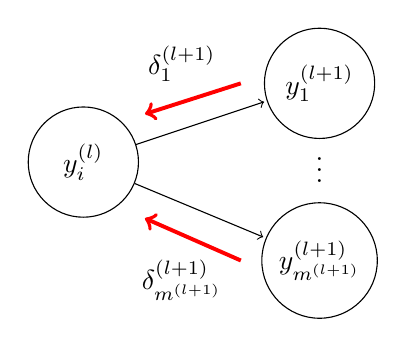
\begin{tikzpicture}[shorten >=1pt]
      		\tikzstyle{unit}=[draw,shape=circle,minimum size =1.4cm]

       	\node[unit](i) at (0,1){$y_i^{(l)}$};
        	\node[unit](k1) at (3,2){$y_1^{(l+1)}$};
		\node at (3, 1){$\vdots$};
		\node[unit](km) at (3,-0.25){$y_{m^{(l+1)}}^{(l+1)}$};
		
		\node at (1.25,2.25){$\delta_1^{(l+1)}$};
		\node at (1.25,-0.5){$\delta_{m^{(l+1)}}^{(l+1)}$};

        	\draw[->] (i) -- (k1);
		\draw[->] (i) -- (km);
		
		\draw[->,red,line width=0.05cm] (2,-0.25) -- (0.75,0.3);
		\draw[->,red,line width=0.05cm] (2,2) -- (0.75,1.6);
    	\end{tikzpicture}
	\caption[Backpropagation of errors through the network.]{Once evaluated for all output units, the errors $\delta_i^{(L+1)}$ can be propagated backwards according to equation~\eqref{eq:hidden-delta}. The derivatives of all weights in layer $l$ can then be determined using equation~\eqref{eq:derivative}.}.
	\label{fig:error-backpropagation}
\end{SCfigure}

Considering the $i^\text{th}$ hidden unit within an arbitrary hidden layer $l$ we write
\begin{align}
\label{eq:evaluate-derivative}
\frac{\partial E_n}{\partial w_{ij}^{(l)}} \underset{rule}{\overset{\text{chain-}}{=}} \frac{\partial E_n}{\partial z_i^{(l)}} \frac{\partial z_i^{(l)}}{\partial w_{ij}^{(l)}}
\end{align}
and notice that the second factor in equation \eqref{eq:evaluate-derivative} takes the same form as in equation \eqref{eq:output-second-factor}:
\begin{align}
\frac{\partial z_i^{(l)}}{\partial w_{ij}^{(l)}} = \frac{\partial}{\partial w_{ij}^{(l)}} \left[\sum _{k = 0} ^{m^{(l-1)}} w_{ik}^{(l)}y_k^{(l-1)}\right] = y_j^{(l-1)}\onedot
\end{align}
Thus, only the error $\delta _i ^{(l)}$ changes. Using the chain rule we get
\begin{align}
\label{eq:hidden-delta}
\delta _i ^{(l)} := \frac{\partial E_n}{\partial z_i^{(l)}} = \sum _{k = 1} ^{m^{(l+1)}} \frac{\partial E_n}{\partial z_k^{(l+1)}} \frac{\partial z_k^{(l+1)}}{\partial z_i^{(l)}}\onedot
\end{align}
In general, the sum runs over all units directly succeeding the $i^\text{th}$ unit in layer $l$ \cite[p.~242-245]{Bishop:2006}. But we assume that every unit in layer $l$ is connected to every unit in layer $(l+1)$ where we allow the weights $w_{ki}^{(l+1)}$ to vanish. Altogether, by substituting the definition of $\delta _k ^{(l+1)}$ from equation \eqref{eq:hidden-delta} we have
\begin{align}
\label{eq:delta-backpropagation}
\delta _i ^{(l)} = f' \left(z_i^{(l)}\right) \sum _{k = 1} ^{m^{(l+1)}} w_{ik}^{(l+1)} \delta _k ^{(l+1)}\onedot
\end{align}

In conclusion, we have found a recursive algorithm for calculating the gradient $\nabla E_n$ by propagating the errors $\delta _i ^{(L+1)}$ back through the network using equation \eqref{eq:delta-backpropagation} and evaluating the derivatives $\frac{\partial E_n}{\partial w_{ij}^{(l)}}$ using equation \eqref{eq:evaluate-derivative}.

%\begin{Alg}[Error Backpropagation]
%\begin{enumerate}[1.]
%\item Propagate the input value $x_n$ through the network to get the actual input and output of all units.
%\item Calculate $\delta _j ^{(L+1)}$ for all output units and determine $\delta _j ^{(l)}$ for all hidden layers $l$ by using backpropagation:
%\begin{align}
%\label{eq:delta-hidden}
%\delta _j ^{(l)} = f' (z_j^{(l)}) \sum _{k = 1} ^{m^{(l+1)}} w_{ik}^{(l+1)} \delta _k ^{(l+1)}
%\end{align}
%\item Calculate the required derivatives:
%\begin{align}
%\frac{\partial E_n}{\partial w_{ji}^{(l)}} = \delta _j ^{(l)} y_i^{(l-1)}
%\end{align}
%\end{enumerate}
%\end{Alg}

\subsubsection{Efficiency}

The number of operations required for error backpropagation scales with the total number of weights $W$ and the number of units. Considering a sufficiently large multilayer perceptron such that every unit in layer $l$ is connected to every unit in layer $(l+1)$ the cost of propagating an input value through the network is dominated by $W$. Here we neglect the evaluation cost of the activation functions. Because of the weighted sum in equation~\eqref{eq:hidden-delta}, backpropagating the error is dominated by $W$, as well. This leads to an overall effort linear in the total number of weights: $\mathcal{O}(W)$ \cite[p.~246-247]{Bishop:2006}.

\subsection{The Hessian}

Following \cite{Bishop:1992} we derive an algorithm which allows us to evaluate the Hessian exactly by forward and backward propagation. Again, we assume differentiable activation functions within a multilayer perceptron. 

We start by picking two weights $w_{ij}^{(p)}$ and $w_{rs}^{(l)}$ where we assume the layer $p$ to come before layer $l$, that is $p \leq l$. The case where $p > l$ will follow by the symmetry of the Hessian \cite{Bishop:1992}. Figure \ref{fig:hessian} illustrates this setting for $p < (l - 1)$.
\begin{SCfigure}[\sidecaptionrelwidth][t!]
	\centering
	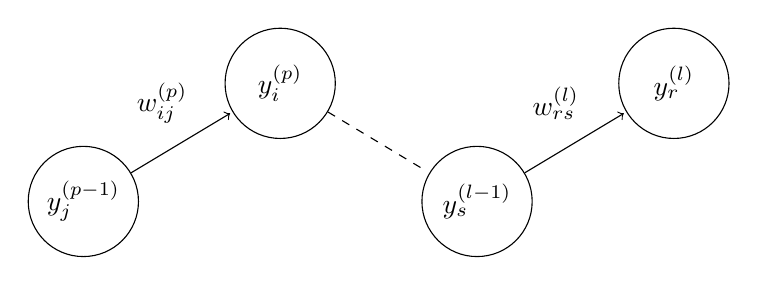
\begin{tikzpicture}[shorten >=1pt]
      		\tikzstyle{unit}=[draw,shape=circle,minimum size =1.4cm]

       	\node[unit](j) at (0,0){$y_j^{(p-1)}$};
        	\node[unit](i) at (2.5,1.5){$y_i^{(p)}$};

		\node[unit](s) at (5,0){$y_s^{(l-1)}$};
		\node[unit](r) at (7.5,1.5){$y_r^{(l)}$};
		
		\node at (1,1.25) {$w_{ij}^{(p)}$};
		\node at (6,1.25) {$w_{rs}^{(l)}$};
		
        	\draw[->] (j) -- (i);
        	\draw[dashed] (i) -- (s);
		\draw[->] (s) -- (r);
    	\end{tikzpicture}
	\caption[Exact evaluation of the Hessian.]{To derive an algorithm for evaluating the Hessian we consider two weights $w_{ij}^{(p)}$ and $w_{rs}^{(l)}$ where we assume that $p \leq l$. This figure illustrates the case when $p < (l - 1)$.}
	\label{fig:hessian}
\end{SCfigure}
As the error $E_n$ is only depending on $w_{ij}^{(p)}$ through the actual input $z_i^{(p)}$ of the $i^\text{th}$ unit in layer $p$ we start by writing
\begin{align}
\frac{\partial^2 E_n}{\partial w_{ij}^{(p)} \partial w_{rs}^{(l)}} \underset{rule}{\overset{\text{chain-}}{=}} \frac{\partial z_i^{(p)}}{\partial w_{ij}^{(p)}} \frac{\partial}{\partial z_i^{(p)}} \left(\frac{\partial E_n}{\partial w_{rs}^{(l)}}\right)\notag\\\overset{\eqref{eq:output-second-factor}}{=} y_j^{(p - 1)} \frac{\partial}{\partial z_i^{(p)}} \left(\frac{\partial E_n}{\partial w_{rs}^{(l)}}\right)\onedot
\end{align}
Now we remember the definition of $\delta _r ^{(l)}$ in equation \eqref{eq:hidden-delta} and add two more definitions:
\begin{align}
\label{eq:g-b}
g_{si} ^{(l - 1,p)} := \frac{\partial z_s^{(l - 1)}}{\partial z_i^{(p)}} \text{ and } b_{ri} ^{(l,p)} := \frac{\partial \delta_r ^{(l)}}{\partial z_i^{(p)}}\onedot
\end{align}
As $E_n$ is depending on $w_{rs}^{(l)}$ only through the value of $z_r^{(l)}$ we use the chain rule and write
\begin{align}
\frac{\partial^2 E_n}{\partial w_{ij}^{(p)} \partial w_{rs}^{(l)}} & = \frac{\partial}{\partial z_i^{(p)}} \left[y_j^{(p - 1)} \frac{\partial z_r^{(l)}}{\partial w_{rs}^{(l)}} \frac{\partial E_n}{\partial z_r^{(l)}}\right]\notag\\
 & = \frac{\partial}{\partial z_i^{(p)}} \left[y_j^{(p - 1)}   y_s^{(l-1)}\frac{\partial E_n}{\partial z_r^{(l)}}\right]\notag\\
 & \overset{\eqref{eq:hidden-delta}}{=} \frac{\partial}{\partial z_i^{(p)}} \left[y_j^{(p - 1)} y_s^{(l-1)}\delta_r^{(l)}\right]\onedot
\end{align}
Because the output $y_j^{(p-1)}$ of the $j^\text{th}$ unit in layer $(p - 1)$ is not depending on $z_i^{(p)}$, we can use the product rule and plug in the definitions from equation \eqref{eq:g-b}:
\begin{align}
\label{eq:hessian-evaluation}
\frac{\partial^2 E_n}{\partial w_{ij}^{(p)} \partial w_{rs}^{(l)}} & \underset{rule}{\overset{\text{product-}}{=}} y_j^{(p-1)} f'\left(z_s^{(l-1)}\right) \frac{\partial z_s^{(l-1)}}{\partial z_i^{(p)}} + y_j^{(p-1)} y_s^{(l-1)} \frac{\partial \delta _r ^{(l)}}{\partial z_i ^{(p)}}\notag\\
& \overset{\eqref{eq:g-b}}{=} y_j^{(p-1)} f'\left(z_s^{(l-1)}\right) g_{si}^{(l-1,p)} + y_j^{(p-1)} y_s^{(l-1)} b_{pi}^{(l,p)}\onedot
\end{align}

Following this derivation, Bishop suggests a simple algorithm to evaluate the $g_{si}^{(l-1,p)}$ and the $b_{ri}^{(l,p)}$ by forward and backward propagation. Using the chain rule we can write
\begin{align}
g_{si} ^{(l - 1,p)} \overset{\eqref{eq:g-b}}{=} \frac{\partial z_s^{(l - 1)}}{\partial z_i^{(p)}} & \underset{rule}{\overset{\text{chain-}}{=}} \sum _{k = 1} ^{m^{(l - 2)}} \frac{\partial z_s^{(l-1)}}{\partial z_k^{(l - 2)}} \frac{\partial z_k^{(l - 2)}}{\partial z_i^{(p)}}\notag\\
& = \sum _{k = 1} ^{m^{(l - 2)}} f'\left(z_k^{(l - 2)}\right) w_{sk}^{(l - 1)} g_{ki}^{(l-2)}\onedot
\end{align}
Initially we set $g_{ii}^{p,p} = 1$ and $g_{si}^{l,p} = 0$ for $l \leq p$. Thus, the $g_{si}^{(l-1,p)}$ can be obtained by forward propagating them through the network. Using the definition of $\delta_r^{(l)}$ from equation \eqref{eq:hidden-delta}, the product rule and the definitions from equation \eqref{eq:g-b} we write
\begin{align}
\label{eq:backpropagation-b}
b_{ri} ^{(l,p)} & \overset{\eqref{eq:g-b}}{=} \frac{\partial \delta_r ^{(l)}}{\partial z_i^{(p)}} \overset{\eqref{eq:hidden-delta}}{=} \frac{\partial f'\left(z_r^{(l)}\right) \left(\sum _{k = 1}^{m^{(l+1)}} w_{kr}^{(l+1)} \delta_k^{(l+1)}\right)}{\partial z_i^{(p)}}\notag\\
& \underset{rule}{\overset{\text{product-}}{=}} f''\left(z_r^{(l)}\right) \frac{\partial z_r^{(l)}}{\partial z_i^{(p)}} \left[ \sum _{k = 1}^{m^{(l+1)}} w_{kr}^{(l+1)} \delta _k^{(l+1)}\right] + f'\left(z_r^{(l)}\right) \left[\sum _{k = 1} ^{m^{(l+1)}} w_{kr}^{(l+1)} \frac{\partial \delta_k^{(l+1)}}{\partial z_i^{(p)}}\right]\notag\\
& \overset{\eqref{eq:g-b}}{=} f''\left(z_r^{(l)}\right) g_{ri}^{(l,p)} \left[ \sum _{k = 1}^{m^{(l+1)}} w_{kr}^{(l+1)} \delta _k^{(l+1)}\right] + f'\left(z_r^{(l)}\right) \left[\sum _{k = 1} ^{m^{(l+1)}} w_{kr}^{(l+1)} b_{ki}^{(l+1,p)}\right]\onedot
\end{align}
Using equation \eqref{eq:backpropagation-b} we can backpropagate the $b_{ri}^{(l,p)}$ after evaluating $b_{ki}^{(L+1,p)}$ for all output units $k$:
\begin{align}
b_{ki}^{(L+1,p)} & \overset{\eqref{eq:g-b}}{=} \frac{\partial \delta_k^{(L+1)}}{\partial z_i^{(p)}} \overset{\eqref{eq:hidden-delta}}{=} \frac{\partial \left(\frac{\partial E_n}{\partial z_k^{(L+1)}}\right)}{\partial z_i^{(p)}}\notag\\
& = \frac{\partial^2 E_n}{\partial^2 z_k^{(L+1)}} \frac{\partial z_k^{(L+1)}}{\partial z_i^{(p)}} = \frac{\partial^2 E_n}{\partial^2 z_k^{(L+1)}} g_{ki} ^{(L+1,p)}\notag\\
& = g_{ki}^{(L+1),p)} \left[f''\left(z_k^{(L+1)}\right) \frac{\partial E_n}{\partial y_k^{(L+1)}} + f'\left(z_k^{(L+1)}\right) \frac{\partial ^2 E_n}{\partial \left(y_k^{(L+1)}\right)^2}\right]\onedot
\end{align}
The errors $\delta_r^{(l)}$ can be evaluated as seen in section \ref{subsec:error-backpropagation} using error backpropagation.

Altogether, we are able to evaluate the Hessian of $E_n$ by forward propagating the $g_{si}^{(l-1,p)}$ and backward propagating the $b_{ri}^{(l,p)}$ as well as the errors $\delta_r^{(l)}$ \cite{Bishop:1992}.

% \subsubsection{Diagonal Approximation}
%
% For several reasons it may be of importance to efficiently evaluate an approximation of the hessian matrix. We discuss an diagonal approximation of the hessian matrix as it is used for regularization using the Optimal Brain Damage algorithm \cite{LeCunDenkerSolla:1990}. Therefore, using the chain rule we write:
%\begin{align}
%\frac{\partial^2 E_n}{\partial w_{ij^2}^{(l)}} & = \frac{\partial}{\partial w_{ij}^{(l)}} \left[ \frac{\partial E_n}{\partial y_i^{(l)}} \frac{\partial y_i^{(l)}}{\partial w_{ij}^{(l)}} \right]\notag\\
%& = \frac{\partial}{\partial w_{ij}^{(l)}} \left[ \frac{\partial E_n}{\partial y_i^{(l)}} f'\left(z_i^{(l)}\right) \frac{\partial z_i^{(l)}}{\partial w_{ij}^{(l)}} \right]\notag\\
%& = \frac{\partial^2 E_n}{\partial w_{ij}^{(l)} \partial y_i^{(l)}} f'\left(z_i^{(l)}\right) y_j^{(l-1)} + \frac{\partial E_n}{\partial y_j^{(l)}} f''\left(z_i^{(l)}\right)\left(y_j^{(l-1)}\right)^2\onedot
%\end{align}

\subsubsection{Efficiency}

We require one step of forward propagation and backward propagation per unit within the network. Again, assuming a sufficiently large network such that the number of weights $W$ dominates the network, the evaluation of equation \eqref{eq:hessian-evaluation} requires $\mathcal{O}(W^2)$ operations.

\subsection{Regularization}

Now we focus on the ability of generalization. We saw that theoretically a neural network with a sufficiently large number of hidden units can model every continuous target function. The ability of a network to generalize can be observed using unseen test data not used for training, usually called a validation set. If the trained approximation of the target function works well for the validation set the network is said to have good generalization capabilities \cite[p.~227-228]{Haykin:2005}. Overtraining of the network may result in over-fitting of the training set, that is the network memorizes the training set but performs very poorly on the validation set \cite[p.~227-228]{Haykin:2005}.

Regularization tries to avoid over-fitting and to give a better generalization performance. This can be achieved by controlling the complexity of the network which is mainly determined by the number of hidden units. The simplest form of regularization is adding a regulizer to the error function such that
\begin{align}
\hat{E}(w) = E(w) + \eta P(w)
\end{align}
where $P(w)$ is a penalty term which tries to influence the form and complexity of the solution \cite[p.~338]{Bishop:1995}.

\begin{SCfigure}[\sidecaptionrelwidth][t!]
	\centering
    	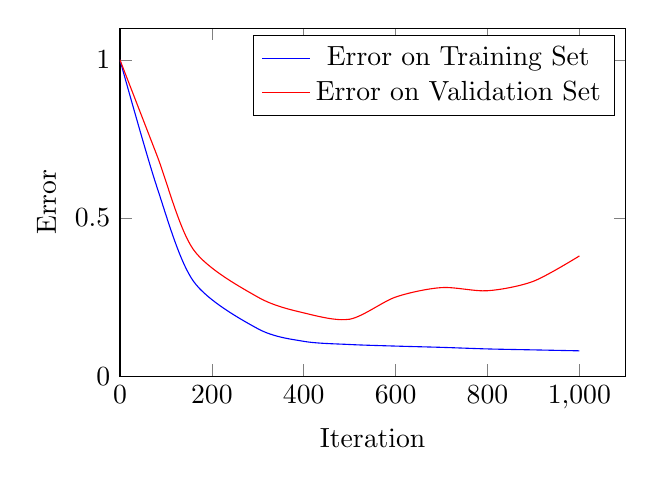
\begin{tikzpicture}
		\begin{axis}[height=6cm,width=8cm,ylabel=Error,xlabel=Iteration,xmin=0,ymin=0]
			\addplot[blue,smooth] coordinates{(0,1)(80,0.6)(160,0.3)(300,0.15)(400,0.11)(500,0.1)(600,0.095)(700,0.091)(800,0.086)(900,0.083)(1000,0.08)};
			\addlegendentry{Error on Training Set}
			\addplot[red,smooth] coordinates{(0,1)(80,0.7)(160,0.4)(300,0.25)(400,0.2)(500,0.18)(600,0.25)(700,0.28)(800,0.27)(900,0.3)(1000,0.38)};
			\addlegendentry{Error on Validation Set}
		\end{axis}
	\end{tikzpicture}
    	\caption[Early stopping based on a validation set.]{The error on the validation set (red) is usually getting larger when the network begins to overfit the training set. Thus, although the error on the training set (blue) is decreasing monotonically, we may want to stop training early to avoid overfitting.}
    	\label{fig:early-stopping}
\end{SCfigure}

\subsubsection{L2-Regularization}

Large weights result in an approximation with poor generalization capabilities. Therefore we try to penalize large weights such that we have \cite[p.~338-343]{Bishop:1995}:
\begin{align}
\hat{E}(w) = E(w) + \eta w^T w.
\end{align}
This regulizer is also referred to as weight decay. For understanding why this regulizer is called weight decay, we consider the derivative of the error function $\hat{E}$ which is given by
\begin{align}
\nabla \hat{E} = \nabla E + \eta w\onedot
\end{align}
Neglecting $\nabla E$ and considering gradient descent learning the change in $w$ with respect to the iteration step $t$ can be described as
\begin{align}
\label{eq:weight-decay-derivative}
\frac{\partial}{\partial t} w[t] = - \gamma \eta w[t]\onedot
\end{align}
Equation \eqref{eq:weight-decay-derivative} has the solution $w[t] = w[0] e^{- \gamma \eta t}$ such that the weights tend exponentially to zero -- giving the method its name \cite[p.~338-340]{Bishop:1995}. While weight decay represents L2-regularization we could also consider L1-regularization.

\subsubsection{Early Stopping}

Early stopping describes the approach to stop training before gradient descent has finished. The error on the training set is usually monotonically decreasing with respect to the iteration number. For unseen data the error is usually much higher and not monotonically decreasing. It tends to get larger when we reach a state of over-fitting. Therefore, it seems reasonable to stop training at a point where the error on the validation set reaches a minimum \cite[p.~343-345]{Bishop:1995}. This is illustrated in figure \ref{fig:early-stopping}.

% \subsubsection{Training invariances}

% Additionally to the training data we often have prior knowledge about desired mapping of the neural network. This includes invariances -- the output should be unchanged if the data istransformed in some specified way.

\newpage

\section{Pattern Classification}
\label{sec:pattern-recognition}

In this section we have a closer look on pattern classification. The classification problem can be defined as follows: Given a $D$-dimensional input vector $x$ assign it to one of $C$ discrete classes. We refer to a given class by its number $c$ which lies in the range $1 \leq c \leq C$. The input vector $x$ is also called pattern or observation.

\subsection{Statistical Background}

Using a statistical approach we assume the pattern $x$ and the class $c$ to be random variables. Then $p(x)$ is the probability that we observe the pattern $x$ and $p(c)$ is the probability that we observe a pattern belonging to class $c$ \cite[p.~108-109]{Ney:1995}.

The classification task is to assign a pattern $x$ to its corresponding class. This can be accomplished by considering the class-conditional probability $p(c|x)$, that is the probability of pattern $x$ belonging to class $c$ \cite[p.~108-109]{Ney:1995}. By applying Bayes' theorem we can rewrite the class-conditional probability to give 
\begin{align}
p(c|x) = \frac{p(x|c) p(c)}{p(x)}\onedot
\end{align}
Then the class-conditional probability can be interpreted as posterior probability where $p(c)$ is the prior probability. The prior probability represents the probability of class $c$ before making an observation. The posterior probability describes the probability of class $c$ after observing the pattern $x$. \cite[p.~38-39]{Bishop:2006}.

\subsection{Bayes' Decision Rule}

Given the posterior probabilities $p(c|x)$ for all classes $c$ we can determine the class of $x$ using a decision rule. But we want to avoid decision errors. A decision error occurs if an observation vector $x$ is assigned to the wrong class. Bayes' decision rule given by
\begin{align}
c:\mathbb{R}^D \rightarrow \{1, \ldots, C\}, x \mapsto \underset{1 \leq c \leq C}{argmax} \left\{p(c | x)\right\}
\end{align}
results in a minimum number of decision errors \cite[p.~109]{Ney:1995}. But it assumes the true posterior probabilities to be known.

In practice the posterior probabilities $p(c|x)$ are unknown. Therefore, we may model the probability $p(c|x)$ directly (or indirectly by modeling $p(x | c)$ first) in the means of a so called model distribution $q_\theta(c|x)$ which depends on some parameters~$\theta$ \cite[p.~637-638]{Ney:2003}. Then we apply the model-based decision rule given by
\begin{align}
\label{eq:decision-rule}
c_\theta:\mathbb{R}^D \rightarrow \{1, \ldots, C\}, x \mapsto \underset{1 \leq c \leq C}{argmax} \left\{q_\theta(c | x)\right\}\onedot
\end{align}
Here we use the model distribution and, thus, the decision rule is fully dependent on the parameters $\theta$ \cite[p.~638]{Ney:2003}.

% In another approach we first model the class-conditional probabilities $p(x | c)$ using a model distribution $q_\theta (x | c)$. When assuming the prior distribution $p(c)$ to be known we can express the posterior probability by using  Bayes' theorem \cite[p.~337-638]{Ney:2003}:
%\begin{align}
%p(c | x) = \frac{q_\theta (x | c) p(c)}{p(x)} = \frac{q_\theta (x | c) p(c)}{\sum _{c = 1} ^C q_\theta (x | c) p(x)}\onedot
%\end{align}
% This approach is also known as generative model because by modeling $p(x | c)$ we are able to generate new patterns for each class \cite[p.~43]{Bishop:2006}.

\subsection{Maximum Likelihood Estimation}

Using a maximum likelihood approach we can estimate the unknown parameters of the model distribution. Therefore, we assume that the posterior probabilities are given by the model distribution $q_\theta(c | x)$ and the patterns $x_n$ are drawn independently from the distribution $q_\theta(c|x)$. We say the data points $x_n$ are independent and identically distributed \cite[p.~85-88]{DudaHartStork:2001}. Then the likelihood function is given by
\begin{align}
\mathcal{L}(\theta) = \prod _{n=1} ^N q_\theta(c_n | x_n)\onedot
\end{align}
where $c_n$ denotes the corresponding class of pattern $x_n$. We then want to maximize $\mathcal{L}(\theta)$. This is equivalent to minimizing the negative log-likelihood function which is given by
\begin{align}
- \log(\mathcal{L}(\theta)) = - \sum _{n=1} ^N \log(q_\theta(x_n | c))\onedot
\end{align}
Then, we can use the negative log-likelihood function as error function to train a neural network. The sum-of-squared error function and the cross-entropy error function can both be motivated using a maximum likelihood approach. We derive only the cross-entropy error function in the next section.

% \subsection{Binary Classification}
%
% As example we follow \cite[p.~234-235]{Bishop:2006} and consider binary classification. As in section \ref{sec:network-training} we assume a data set $T = \{(x_n, t_n) : 1 \leq n \leq N\}$ to be given where $t_n = c = 1$ refers to the first class whereas $t_n = c = 0$ refers to the second class.

% We model the posterior probability $p(c | x)$ in the means of a Bernoulli distribution
%\begin{align}
%q_\theta(c | x) = \theta^c (1 - \theta)^{1-c}
%\end{align}
% where $\theta$ is the probability of $x$ belonging to class $c = 1$. Then we have a single parameter~$\theta$. Now we can apply maximum likelihood estimation by assuming the training set to be a set of independent patterns $x_n$. Then, the likelihood function is given by
%\begin{align}
%\mathcal{L}(\theta) = \prod _{n = 1} ^N q_\theta(x_n | c) = \prod _{n = 1} ^N \theta ^{c_n} (1 - \theta)^{1 - c_n}\onedot
%\end{align}
%
% To derive an appropriate error function to train a neural network we consider the negative log-likelihood function:
%\begin{align}
%\label{eq:binary-classification-nloglikelihood}
%- \log(\mathcal{L}(\theta) & = - \sum _{n = 1} ^N \log\left(\theta ^{c_n} (1 - \theta)^{1 - c_n}\right)\notag\\
%& = - \sum _{n = 1} ^N c_n \log(\theta) + (1 - c_n) \log(1 - \theta) \onedot
%\end{align}
% We then consider the probability $\theta$ to be given by the network output. For this purpose we choose a sigmoidal activation function for the single output unit such that:
%\begin{align}
%y(x,w) = \frac{1}{1 + \exp(-z)} \in [0,1]
%\end{align}
% where $z$ is the actual input of the output unit as used in section \ref{sec:neural-networks}. By substituting $\theta = y(x,w)$ into equation \eqref{eq:binary-classification-nloglikelihood} we get the error function
%\begin{align}
%E(w) = - \sum _{n = 1} ^N c_n \log(y(x_n,w)) (1 - c_n) \log(1 - y(x_n,w))
%\end{align}
% which can be interpreted as a sepcial case of the cross-entropy error function introduced in section \ref{subsec:error-measures}.

\subsubsection{Derivation of Cross-Entropy}

We follow \cite[p.~232-236]{Bishop:2006} and consider the multiclass\footnote{Generally, we distinguish the binary classification problem in the case of $C = 2$ and the multiclass classification problem for $C > 2$.} classification problem. The target values $t_n$ follow the $1$--of--$C$ encoding scheme, that is the $i^\text{th}$ entry of $t_n$ equals $1$ iff the pattern $x_n$ belongs to class $i$.

We interpret the output of the neural network as the posterior probabilities
\begin{align}
p(c | x) = y_c(x,w)\onedot
\end{align}
The posterior probability for class $c$ can then be written as
\begin{align}
\label{eq:multiclass-posterior}
p(c | x) = \frac{p(x | c) p(c)}{\sum _{k = 1} ^C p(x | k) p(k)}\onedot
\end{align}
As output activation function we use the softmax function such that we can rewrite equation \eqref{eq:multiclass-posterior} to give
\begin{align}
p(c | x) = \frac{\exp({z_c})}{\sum _{k = 1} ^c \exp({z_k})} \text{ with } z_k = \log(p(k | x) p(k))\onedot
\end{align}
Here we model the posteriors in the means of the network output. This means that the parameters of the model distribution are given by the weights of the network. Given the probabilities $p(c | x)$ the maximum likelihood function takes the form
\begin{align}
\mathcal{L} (w) = \prod _{n = 1} ^N \prod _{c} ^C p(c | x_n)^{t_{nc}} =  \prod _{n = 1} ^N \prod _{c = 1} ^C y_c(x_n,w)^{t_{nc}}
\end{align}
and we can derive the error function $E(w)$ which is given by the cross-entropy error function already introduced in section \ref{subsec:error-measures}:
\begin{align}
E(w) = - \log(\mathcal{L}(w)) = - \sum _{n = 1} ^N \sum _{c = 1} ^C t_{nc} ln(y_c(w, x_n))\onedot
\end{align}
% In this case we directly modeled the posterior probabilities in the means of the network output. Thus the likelihood function estimates the parameters $w$ of the neural network rather than parameters for a model distribution.

\subsection{Application: Recognizing Handwritten Digits}

\begin{figure}
	\centering
	\subfigure[100 units, $\gamma = 0.5$]{
		\includegraphics[width=0.2\textwidth]{images/100-500-0,5.png}
	}
	\subfigure[300 units, $\gamma = 0.5$]{
		\includegraphics[width=0.2\textwidth]{images/100-500-0,5-300units.png}
	}
	\subfigure[400 units, $\gamma = 0.5$]{
		\includegraphics[width=0.2\textwidth]{images/100-500-0,5-400units.png}
	}
	\subfigure[500 units, $\gamma = 0.5$]{
		\includegraphics[width=0.2\textwidth]{images/100-500-0,5-500units.png}
	}
	\subfigure[600 units, $\gamma = 0.5$]{
		\includegraphics[width=0.2\textwidth]{images/100-500-0,5-600units.png}
	}
	\subfigure[700 units, $\gamma = 0.5$]{
		\includegraphics[width=0.2\textwidth]{images/100-500-0,5-700units.png}
	}
	\subfigure[750 units, $\gamma = 0.1$]{
		\includegraphics[width=0.2\textwidth]{images/100-500-0,1-750units.png}
	}
	\subfigure[800 units, $\gamma = 0.1$]{
		\includegraphics[width=0.2\textwidth]{images/100-500-0,1-800units.png}
	}
	\caption[Error on the training set during training.]{The error during training for different learning rates $\gamma$ and numbers of hidden units. The two-layer perceptron was trained with a batchsize of $100$ randomly chosen images iterated $500$ times. The error was measured using the sum-of-squared error function and plotted after each iteration.}
\end{figure}

Based on the MNIST dataset (available online at \href{http://yann.lecun.com/exdb/mnist/}{http://yann.lecun.com/exdb/mnist/}) we want to train a two-layer perceptron to recognize handwritten digits. The dataset provides a training set of $60,000$ images and a validation set of $10,000$ images. The images have $28 \times 28$ pixels of size and, thus, we may write an image as vector with $28 \cdot 28 = 784$ dimensions. The neural network will be trained using gradient descent for parameter optimization and the sum-of-squared error function. The training procedure is implemented in MatLab.

\subsubsection{Matrix Notation}

For implementing error backpropagation in MatLab it is convenient to introduce a matrix notation. We discuss the general case of a multilayer perceptron with $L$ layers. The output of all units in layer $l$ and their actual input can both be combined in vectors:
\begin{align}
y^{(l)} := \left( y_i ^{(l)} \right)_{i = 1}^{m^{(l)}} \text{ and } z^{(l)} := \left( z_i^{(l)} \right)_{i = 1}^{m^{(l)}}\onedot
\end{align}
When combining all weights $w_{ij}^{(l)}$ of layer $l$ in a single weight matrix we can express the propagation of an input vector through the network as several vector matrix products. The weight matrix $W^{(l)}$ is given by
\begin{align}
W^{(l)} := \left(w_{ij}^{(l)}\right)_{i,j = 1}^{m^{(l)},m^{(l-1)}}\onedot
\end{align}
Propagating the output vector of layer $(l - 1)$ denoted by $y^{(l-1)}$ through layer $l$ can then be written as
\begin{align}
y^{(l)} = f\left(W^{(l)}y^{(l-1)}\right)
\end{align}
where $f$ operates element by element. Given the error vector $\delta ^{(l+1)}$ defined as
\begin{align}
\delta^{(l+1)} := \left(\delta_i^{(l+1)}\right)_{i = 1}^{m^{(l+1)}}
\end{align}
for layer $(l+1)$ we can use the transpose of the weight matrix to give
\begin{align}
\delta ^{(l)} = f'(z^{(l)}) \bullet \left(W^{(l)}\right)^{tr} \delta^{(l+1)}
\end{align}
where $f'$ operates element by element and $\bullet$ denotes the component-wise multiplication.

\subsubsection{Implementation and Results}

The MNIST dataset is provided in the IDX file format. To get the images as vector with $784$ dimensions we use two functions \lstinline{loadMNISTImages} and \lstinline{loadMNISTLabels} which can be found online at \href{http://ufldl.stanford.edu/}{http://ufldl.stanford.edu/}.

Appendix \ref{lst:train-two-layer-perceptron} shows the implementation of the training procedure. The activation function and its derivative are passed as parameters. We use the logistic sigmoid, which is shown in appendix \ref{lst:activation-function}, as activation function for both the hidden and the output layer. The number of hidden units and the learning rate are adjustable. The weight matrices for both layers are initialized randomly and normalized afterwards (lines 29 to 35). We apply stochastic training in so called epochs, that is for each epoch we train the network on randomly selected input values (lines 42 to 61). The number of randomly selected input values to use for training is defined by the parameter \lstinline{batchSize}. After each epoch we plot the current error on the same input values as the network was trained on (lines 63 to 73).

For comparing different configurations we use the validation set. The validation procedure, which counts the number of correctly classified images, is shown in appendix \ref{lst:validation}. The accuracy is measured as the quotient of correctly classified images and the total number of images. Figure \ref{fig:results} shows some of the results.

\begin{figure}[t!]
	\centering
	\subfigure[$500$ epochs with batch size $100$.]{
		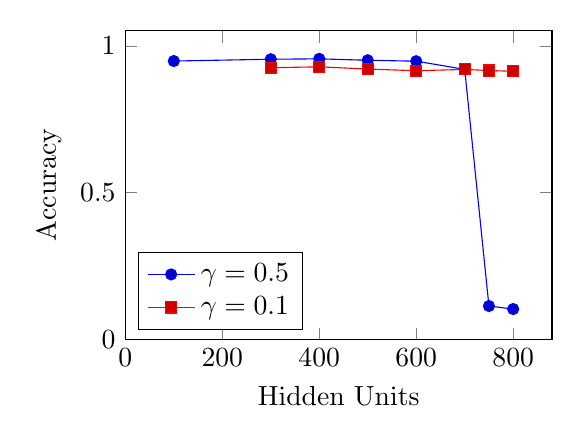
\begin{tikzpicture}
			\begin{axis}[height=5.5cm,width=7cm,ylabel=Accuracy,xlabel=Hidden Units,xmin=0,ymin=0,legend pos=south west]
				\addplot+[blue] coordinates{(100,1-0.0519)(300,1-0.0457)(400,1-0.0444)(500,1-0.0492)(600,1-0.0524)(700,1-0.0801)(750,1-0.8865)(800,1-0.8968)};
				\addlegendentry{$\gamma = 0.5$}
				\addplot+[red] coordinates{(300,1-0.0747)(400,1-0.0716)(500,1-0.0791)(600,1-0.0849)(700,1-0.0804)(750,1-0.0842)(800,1-0.0868)};
				\addlegendentry{$\gamma = 0.1$}
			\end{axis}
		\end{tikzpicture}
		\label{subfig:results-units}
	}
	\subfigure[$500$ epochs with learning rate $\gamma = 0.5$.]{
		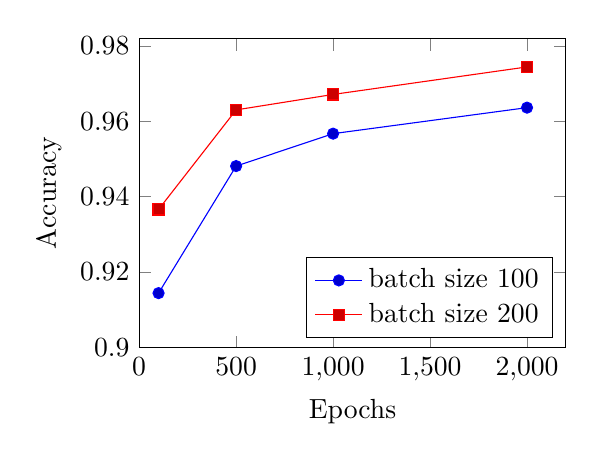
\begin{tikzpicture}
			\begin{axis}[height=5.5cm,width=7cm,ylabel=Accuracy,xlabel=Epochs,xmin=0,ymin=0.9,legend pos=south east]
				\addplot+[blue] coordinates{(100,1-0.0856)(500,1-0.0519)(1000,1-0.0433)(2000,1-0.0364)};
				\addlegendentry{batch size 100}
				\addplot+[red] coordinates{(100,1-0.0634)(500,1-0.0370)(1000,1-0.0329)(2000,1-0.0256)};
				\addlegendentry{batch size 200}
			\end{axis}
		\end{tikzpicture}
		\label{subfig:results-epochs}
	}
	\caption[Results of training a two-layer perceptron using the MNIST dataset.]{Figure \ref{subfig:results-units} plots the achieved accuracy depending on the number of hidden units for a fixed learning rate $\gamma = 0.5$. For $750$ or more units we need to adjust the learning rate in order to ensure convergence. But this may result in slow convergence such that we get worse results for few hidden units. Figure \ref{subfig:results-epochs} shows the impact of increasing the number of epochs. As we would expect, the accuracy increases with rising training set.}
	\label{fig:results}
\end{figure}


\newpage

\section{Conclusion}

In the course of this paper we introduced the general concept of artificial neural networks and had a closer look at the multilayer perceptron. We discussed several activation functions and network topologies and explored the expressive power of neural networks.

Section \ref{sec:network-training} introduced the basic notions of network training. We focussed on supervised training. Therefore, we introduced two different error measure to evaluate the performance of the network in respect to function approximation. To train the network we introduced gradient descent as iterative parameter optimization algorithm as well as Newton's method as second-order optimization algorithm. The weights of the network are adjusted iteratively to minimize the chosen error measure. To evaluate the gradient of the error measure we introduced the error backpropagation algorithm. We extended this algorithm to allow the exact evaluation of the Hessian, as well.

Thereafter, we discussed the classification problem using a statistical approach. Based on maximum likelihood estimation we derived the cross-entropy error measure for multiclass classification. As application we considered digit recognition based on the MNIST dataset using a two-layer perceptron.

Unfortunately this paper is far too short to cover the extensive topic of neural networks and their application in pattern recognition. Especially for network training there are more advanced techniques available (see for example \cite{Bishop:1995}). Instead of the exact evaluation of the Hessian described in \cite{Bishop:1992}, approximations to the Hessian or its inverse are more efficient to compute (for example described in \cite{Bishop:1995}). Based on a diagonal approximation of the Hessian there are advanced regularization methods as for example the Optimal Brain Damage algorithm \cite{LeCunDenkerSolla:1990}.

In conclusion, artificial neural networks are a powerful tool applicable to a wide range of problems especially in the domain of pattern recognition.

\newpage

\begin{appendices}

\section{MatLab Implementation}

\subsection{Logistic Sigmoid and its Derivative}
\begin{lstlisting}[label={lst:activation-function}]
function y = logisticSigmoid(x)
% simpleLogisticSigmoid Logistic sigmoid activation function
% 
% INPUT:
% x     : Input vector.
%
% OUTPUT:
% y     : Output vector where the logistic sigmoid was applied element by
% element.
%

    y = 1./(1 + exp(-x));
end
\end{lstlisting}

\begin{lstlisting}
function y = dLogisticSigmoid(x)
% dLogisticSigmoid Derivative of the logistic sigmoid.
% 
% INPUT:
% x     : Input vector.
%
% OUTPUT:
% y     : Output vector where the derivative of the logistic sigmoid was
% applied element by element.
%
    y = logisticSigmoid(x).*(1 - logisticSigmoid(x));
end
\end{lstlisting}

\subsection{Training Procedure}
\begin{lstlisting}[label={lst:train-two-layer-perceptron}]
function [hiddenWeights, outputWeights, error] = trainStochasticSquaredErrorTwoLayerPerceptron(activationFunction, dActivationFunction, numberOfHiddenUnits, inputValues, targetValues, epochs, batchSize, learningRate)
% trainStochasticSquaredErrorTwoLayerPerceptron Creates a two-layer perceptron
% and trains it on the MNIST dataset.
%
% INPUT:
% activationFunction             : Activation function used in both layers.
% dActivationFunction            : Derivative of the activation
% function used in both layers.
% numberOfHiddenUnits            : Number of hidden units.
% inputValues                    : Input values for training (784 x 60000)
% targetValues                   : Target values for training (1 x 60000)
% epochs                         : Number of epochs to train.
% batchSize                      : Plot error after batchSize images.
% learningRate                   : Learning rate to apply.
%
% OUTPUT:
% hiddenWeights                  : Weights of the hidden layer.
% outputWeights                  : Weights of the output layer.
% 

    % The number of training vectors.
    trainingSetSize = size(inputValues, 2);
    
    % Input vector has 784 dimensions.
    inputDimensions = size(inputValues, 1);
    % We have to distinguish 10 digits.
    outputDimensions = size(targetValues, 1);
    
    % Initialize the weights for the hidden layer and the output layer.
    hiddenWeights = rand(numberOfHiddenUnits, inputDimensions);
    outputWeights = rand(outputDimensions, numberOfHiddenUnits);
    
    hiddenWeights = hiddenWeights./size(hiddenWeights, 2);
    outputWeights = outputWeights./size(outputWeights, 2);
    
    n = zeros(batchSize);
    
    figure; hold on;

    for t = 1: epochs
        for k = 1: batchSize
            % Select which input vector to train on.
            n(k) = floor(rand(1)*trainingSetSize + 1);
            
            % Propagate the input vector through the network.
            inputVector = inputValues(:, n(k));
            hiddenActualInput = hiddenWeights*inputVector;
            hiddenOutputVector = activationFunction(hiddenActualInput);
            outputActualInput = outputWeights*hiddenOutputVector;
            outputVector = activationFunction(outputActualInput);
            
            targetVector = targetValues(:, n(k));
            
            % Backpropagate the errors.
            outputDelta = dActivationFunction(outputActualInput).*(outputVector - targetVector);
            hiddenDelta = dActivationFunction(hiddenActualInput).*(outputWeights'*outputDelta);
            
            outputWeights = outputWeights - learningRate.*outputDelta*hiddenOutputVector';
            hiddenWeights = hiddenWeights - learningRate.*hiddenDelta*inputVector';
        end;
        
        % Calculate the error for plotting.
        error = 0;
        for k = 1: batchSize
            inputVector = inputValues(:, n(k));
            targetVector = targetValues(:, n(k));
            
            error = error + norm(activationFunction(outputWeights*activationFunction(hiddenWeights*inputVector)) - targetVector, 2);
        end;
        error = error/batchSize;
        
        plot(t, error,'*');
    end;
end
\end{lstlisting}

\subsection{Validation Procedure}

\begin{lstlisting}[label={lst:validation}]
function [correctlyClassified, classificationErrors] = validateTwoLayerPerceptron(activationFunction, hiddenWeights, outputWeights, inputValues, labels)
% validateTwoLayerPerceptron Validate the twolayer perceptron using the
% validation set.
%
% INPUT:
% activationFunction             : Activation function used in both layers.
% hiddenWeights                  : Weights of the hidden layer.
% outputWeights                  : Weights of the output layer.
% inputValues                    : Input values for training (784 x 10000).
% labels                         : Labels for validation (1 x 10000).
%
% OUTPUT:
% correctlyClassified            : Number of correctly classified values.
% classificationErrors           : Number of classification errors.
% 

    testSetSize = size(inputValues, 2);
    classificationErrors = 0;
    correctlyClassified = 0;
    
    for n = 1: testSetSize
        inputVector = inputValues(:, n);
        outputVector = evaluateTwoLayerPerceptron(activationFunction, hiddenWeights, outputWeights, inputVector);
        
        class = decisionRule(outputVector);
        if class == labels(n) + 1
            correctlyClassified = correctlyClassified + 1;
        else
            classificationErrors = classificationErrors + 1;
        end;
    end;
end

function class = decisionRule(outputVector)
% decisionRule Model based decision rule.
%
% INPUT:
% outputVector      : Output vector of the network.
%
% OUTPUT:
% class             : Class the vector is assigned to.
%

    max = 0;
    class = 1;
    for i = 1: size(outputVector, 1)
        if outputVector(i) > max
            max = outputVector(i);
            class = i;
        end;
    end;
end

function outputVector = evaluateTwoLayerPerceptron(activationFunction, hiddenWeights, outputWeights, inputVector)
% evaluateTwoLayerPerceptron Evaluate two-layer perceptron given by the
% weights using the given activation function.
%
% INPUT:
% activationFunction             : Activation function used in both layers.
% hiddenWeights                  : Weights of hidden layer.
% outputWeights                  : Weights for output layer.
% inputVector                    : Input vector to evaluate.
%
% OUTPUT:
% outputVector                   : Output of the perceptron.
% 

    outputVector = activationFunction(outputWeights*activationFunction(hiddenWeights*inputVector));
end
\end{lstlisting}

\end{appendices}

\addcontentsline{toc}{section}{Literature}
\bibliographystyle{plain}
\bibliography{seminar}

\end{document}